\PassOptionsToPackage{table}{xcolor}
\documentclass{article}
\usepackage[colorlinks]{hyperref}
\usepackage[margin=1.25in]{geometry}
\usepackage{amsmath,amssymb,amsthm,booktabs,tikz}
\usepackage[final]{microtype}
\usepackage{libertine}
\usepackage[varqu]{zi4}
\usepackage[libertine]{newtxmath}
\usepackage[T1]{fontenc}
\usepackage[utf8]{inputenc}
\usepackage{tabto}
\usepackage[normalem]{ulem}

\usetikzlibrary{shapes.multipart}

% Seven colors safe for use color blindness.
% Colors taken from doi:10.1038/nmeth.1618.
\definecolor{cbOrange}{RGB}{230,159,0}
\definecolor{cbSkyBlue}{RGB}{86,180,233}
\definecolor{cbBluishGreen}{RGB}{0,158,115}
\definecolor{cbBlue}{RGB}{0,114,178}
\definecolor{cbVermillion}{RGB}{213,94,0}
\definecolor{cbReddischPurple}{RGB}{204,121,167}
\definecolor{cbYellow}{RGB}{240,228,66}

\theoremstyle{definition}
\newtheorem{problem}{Problem}
\newenvironment{questions}{\begin{enumerate}
\renewcommand{\theenumi}{P\arabic{problem}.\arabic{enumi}}}{\end{enumerate}}
\newcommand{\HL}[1]{\textcolor{cbReddischPurple}{#1}}

\newcommand{\abs}[1]{\lvert #1 \rvert}
\newcommand{\OOG}[1]{\mathord{\sim}#1}
\DeclareMathOperator{\bdiv}{div}

\newcommand{\BigO}[1]{\mathcal{O}\left(#1\right)}
\newcommand{\BigOmega}[1]{\Omega\left(#1\right)}
\newcommand{\BigTheta}[1]{\Theta\left(#1\right)}


\newcommand{\True}{\texttt{true}}
\newcommand{\False}{\texttt{false}}

%% Tikz
\usepackage{tikz}
\usetikzlibrary{arrows.meta,calc,decorations.pathreplacing,shapes.geometric,shapes.multipart,overlay-beamer-styles}
\tikzset{
    >=Stealth,
    dot/.style={circle,scale=0.35,draw=black,fill=black},
    stacked/.style={above,rectangle split,draw,rectangle split parts=#1,font=\strut,rectangle split part fill={none,black!10}},
    centered/.append style={align=center}
}


% Algorithm
\usepackage{algorithmic}
\newcommand{\GETS}{:=}
\newcommand{\VAR}[1]{\textit{#1\/}}
\newcommand{\AName}[1]{\textsc{#1}}
\renewcommand{\algorithmicrequire}{\textbf{Input:}}
\renewcommand{\algorithmicensure}{\textbf{Result:}}
\newcommand{\CMT}[1]{\text{``#1''}}
\renewcommand{\algorithmiccomment}[1]{\CMT{#1}}
\newcommand{\INV}[1]{\emph{inv: } #1}
\newcommand{\VF}[1]{\emph{bf: } #1}
\makeatletter
\newlength{\Algo@MyTabLength}
\newcommand{\AlgoTabTo}[1]{%
    \setlength{\Algo@MyTabLength}{#1}%
    \addtolength{\Algo@MyTabLength}{-\ALC@tlm}%
    \tabto{\Algo@MyTabLength}%
}
\newenvironment{myonlyalgo}[1][0]{
    \vskip 5pt
    \hrule
    \smallskip
    \begin{algorithmic}[1]
    \setcounter{ALC@line}{#1}
}{
    \end{algorithmic}
    \hrule
    \vskip 5pt
}
\newenvironment{myalgo}[2][0]{
    \vskip 5pt
    \hrule
    \smallskip
    \noindent{\textbf{Algorithm} #2\textbf{:}}
    \begin{algorithmic}[1]
    \setcounter{ALC@line}{#1}
}{
    \end{algorithmic}
    \hrule
    \vskip 5pt
}







%% Metadata
\newcommand{\Assignment}[1]{
    \title{\vskip-2em%The standard article.cls package puts 2em whitespace on top of the title, undo this.
           Assignment #1\\{\Large SFWRENG 2CO3: Data Structures and Algorithms--Winter 2023}}}
\newcommand{\Deadline}[1]{
    \author{Deadline: #1}
}
\date{{\normalsize
    Department of Computing and Software\\
    McMaster University
}}

\newcommand{\Warning}[1]{\textbf{\textcolor{red!80!black}{#1}}}
\renewcommand{\labelitemi}{$\blacktriangleright$}

\newcommand{\DEFAULTMSG}{
Please read the \emph{Course Outline} for the general policies related to assignments.
\begin{center}
\Warning{Plagiarism is a \underline{\textit{\vphantom{y}serious academic offense}} and will be handled accordingly.}\\
\Warning{All suspicions will be reported to the \underline{\textit{Office of Academic Integrity}}\\(in accordance with the \href{https://secretariat.mcmaster.ca/app/uploads/Academic-Integrity-Policy-1-1.pdf}{Academic Integrity Policy}).}
\end{center}

This assignment is an \emph{individual} assignment: do not submit work of others. All parts of your submission \emph{must} be your own work and be based on your own ideas and conclusions. Only \emph{discuss or share} any parts of your submissions with your TA or instructor.  You are \emph{responsible for protecting} your work: you are strongly advised to password-protect and lock your electronic devices (e.g., laptop) and to not share your logins with partners or friends! If you \emph{submit} work, then you are certifying that you have completed the work for this assignment by yourself. By submitting work, you agree to automated and manual plagiarism checking of all submitted work.

\emph{Late submission policy}. Late submissions will receive a late penalty of 20\% on the score per day late (with a five hour grace period on the first day, e.g., to deal with technical issues) and submissions five days (or more) past the due date are not accepted. In case of technical issues while submitting, contact the instructor \emph{before} the deadline.}

\newcommand{\SUBMITMSG}{\section*{Assignment Details}
Write a report in which you solve each of the above problems. Your submission:
\begin{enumerate}
\item must be a \texttt{PDF} file;
\item must have clearly labeled solutions to each of the stated problems;
\item must be clearly presented;
\item must \emph{not} be hand-written: prepare your report in \LaTeX{} or in a word processor such as Microsoft Word (that can print or exported to \texttt{PDF}).
\end{enumerate}
\Warning{Submissions that do not follow the above requirements will get a grade of zero.}}

\newcommand{\DEFAULTGRADING}{\section*{Grading}
Each problem counts equally toward the final grade of this assignment.
}

\usepackage{forest}
\usepackage{graphicx}
\definecolor{cbOrange}{RGB}{230,159,0}
\definecolor{cbSkyBlue}{RGB}{86,180,233}
\definecolor{cbBluishGreen}{RGB}{0,158,115}
\definecolor{cbBlue}{RGB}{0,114,178}
\definecolor{cbVermillion}{RGB}{213,94,0}
\definecolor{cbReddischPurple}{RGB}{204,121,167}
\definecolor{cbYellow}{RGB}{240,228,66}
\usetikzlibrary{positioning,matrix, arrows.meta}


\Assignment{2}
\Deadline{February 12, 2023}
\begin{document}
\maketitle
\DEFAULTMSG{}

\begin{problem}
Assume we have a computer with infinite processor cores that can all operate at the same time. In an attempt to sort \emph{as fast as possible}, we make a \emph{parallelized} version of \AName{MergeSort} that uses multiple processor cores at the same time. To achieve this, we change the top-down merge-sort algorithm as follows:
\begin{myalgo}{\AName{ParallelMergeSort}($L[\VAR{start}\dots\VAR{end})$)}
    \IF{$\VAR{start} + 1 < \VAR{end}$}
        \STATE $\VAR{mid} \GETS (start + end) \bdiv 2$.
        \STATE Start \AName{ParallelMergeSort}($L[\VAR{start},\VAR{mid})$) on a fresh processor core $C$.
        \STATE $L_2 \GETS \AName{ParallelMergeSort}(L[\VAR{mid}\dots\VAR{end}))$.
        \STATE Wait until $C$ finished \AName{ParallelMergeSort}($L[\VAR{start},\VAR{mid})$), resulting in $L_1$.
        \RETURN \AName{Merge}($L_1, L_2$).
    \ELSE
        \RETURN $L$.
    \ENDIF
\end{myalgo}
Let $n = \abs{L}$ be the length of the list being sorted by \AName{ParallelMergeSort}.
\begin{questions}
\item Give a recurrence $T(n)$ for the runtime complexity of \AName{ParallelMergeSort} and solve the recurrence $T(n)$ by proving that $T(n) \OOG{e(n)}$ for some expression $e$ that uses $n$.\\
\textbf{Answer:}\\
\begin{center}
\begin{forest}
    for tree={
      draw,
      align=center
    }
    [N
      [$\frac{N}{2}$
        [$\frac{N}{4}$
          [...]
        ]
        [$\frac{N}{4}$
          [...]
        ]
      ]
      [$\frac{N}{2}$
        [$\frac{N}{4}$
            [...]
        ]
        [$\frac{N}{4}$
            [...]
        ]
      ]
    ]
  \end{forest}
  \quad
  \begin{tabular}{ c c c }
    Number & Cost & Total\\
    1 & $N$ & $1*N$\\
    1 & $\frac{N}{2}$ & $1*\frac{N}{2}$\\
    1 & $\frac{N}{4}$ & $1*\frac{N}{4}$\\
    ... & ... & ...\\
    1 & $\frac{N}{2^i}$ & $1*\frac{N}{2^i}$\\
    --- & --- & ---\\
     & & $2N$
  \end{tabular}
\end{center}

As you can see, the tree shows that each step has $\frac{N}{2^i}$ cost. There is only 1 counted as they all occur in parallel, so unlike the cost complexity, the time complexity is as if the step is just run once. When you go to sum up all the steps, you can see that the steps will converge to 2N which is $\sim$ N. Note: $N + \frac{N}{2} + \frac{N}{4} + \frac{N}{8} +... = 2N$. Given N is not always a power of 2, we know that $O(N)$ is upper bounded by 2N and it must be lower bounded by N since the first step will always have a cost of N. This is enough to prove that the algorithm is $\sim N$.

\item Provide a strict bound on the number of processor cores that \AName{ParallelMergeSort} uses (hence, how many different processor cores are used by \AName{ParallelMergeSort} at the same time).\\
\textbf{Answer:}\\
Assumption: When a core calls two parallel MergeSorts, the core will handle one and delegate the other call to a new core.\\

The number of processors is $2^{\log_2 N} = N$. This is because the recurrance tree proves to be $\log_2N$ height and each step has double the processors of the last step. On the last reccurance level, it will terminate as there is only 1 element in the List, so it will hit the else statement (rather than the if condition) and return the List. This is an assumption that N is a power of 2. Given N is not always a power of 2, we know the number of processors is in the range of $2^{\log_2 N-1} <= processors <= N$, which contains the min and max number of processors needed per level on the reccurance tree.
\end{questions}
\end{problem}

\begin{problem}
Consider the following recursive sorting algorithm.
\begin{myalgo}{\AName{WeirdSort}($L$, $\VAR{start}$, $\VAR{end}$)}
    \IF{$\VAR{end} - \VAR{start} = 2$}
        \IF{$L[\VAR{start}] \geq L[\VAR{start} + 1]$}
            \STATE Exchange $L[\VAR{start}]$ and $L[\VAR{start} + 1]$.
        \ENDIF
    \ELSIF{$\VAR{end} - \VAR{start} > 2$}
        \STATE $k \GETS (\VAR{end} - \VAR{start}) \bdiv 3$.
        \STATE \AName{WeirdSort}($L$, $\VAR{start}$, $\VAR{end} - k$).
        \STATE \AName{WeirdSort}($L$, $\VAR{start} + k$, $\VAR{end}$).
        \STATE \AName{WeirdSort}($L$, $\VAR{start}$, $\VAR{end} - k$).
    \ENDIF
\end{myalgo}
Let $n = \abs{L}$ be the length of the list being sorted by \AName{WeirdSort}.

\begin{questions}
\item Is \AName{WeirdSort} a \emph{stable} sort algorithm? If yes, explain why. If no, show why not and indicate whether the algorithm can be made stable.\\
\textbf{Answer:}\\
This is not a stable sort algorithm as in line 2, if the earlier element is equal to the next element, they get swapped. To make this a stable algorithm, change $\geq$ to $>$.
\item Prove via induction that \AName{WeirdSort} will sort list $L$.\\
\textbf{Answer:}\\
% 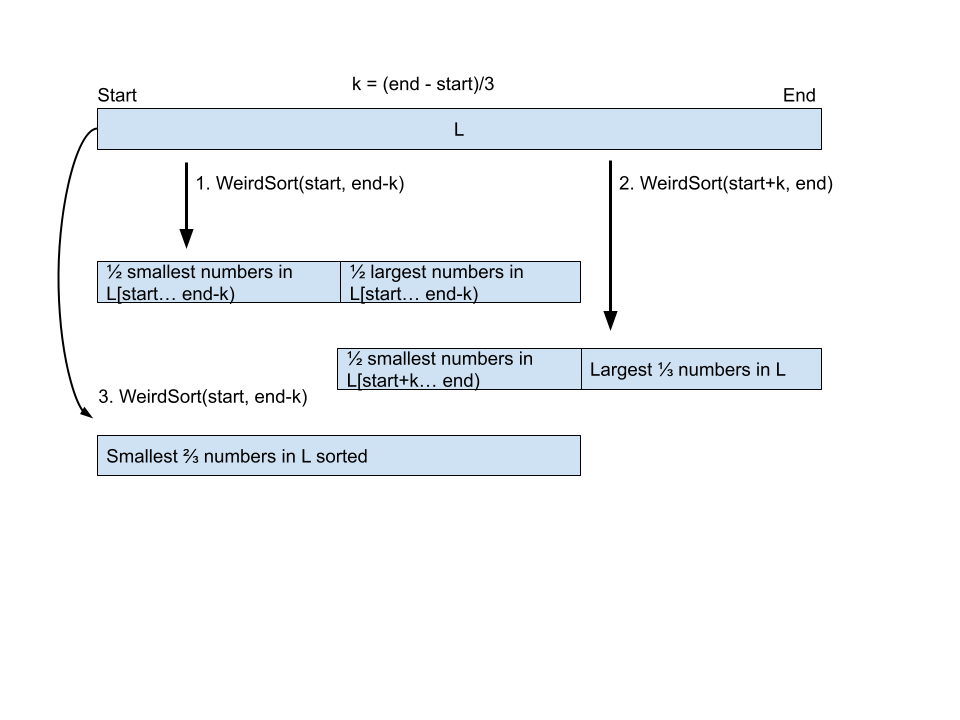
\includegraphics[scale=0.5]{question2.png}

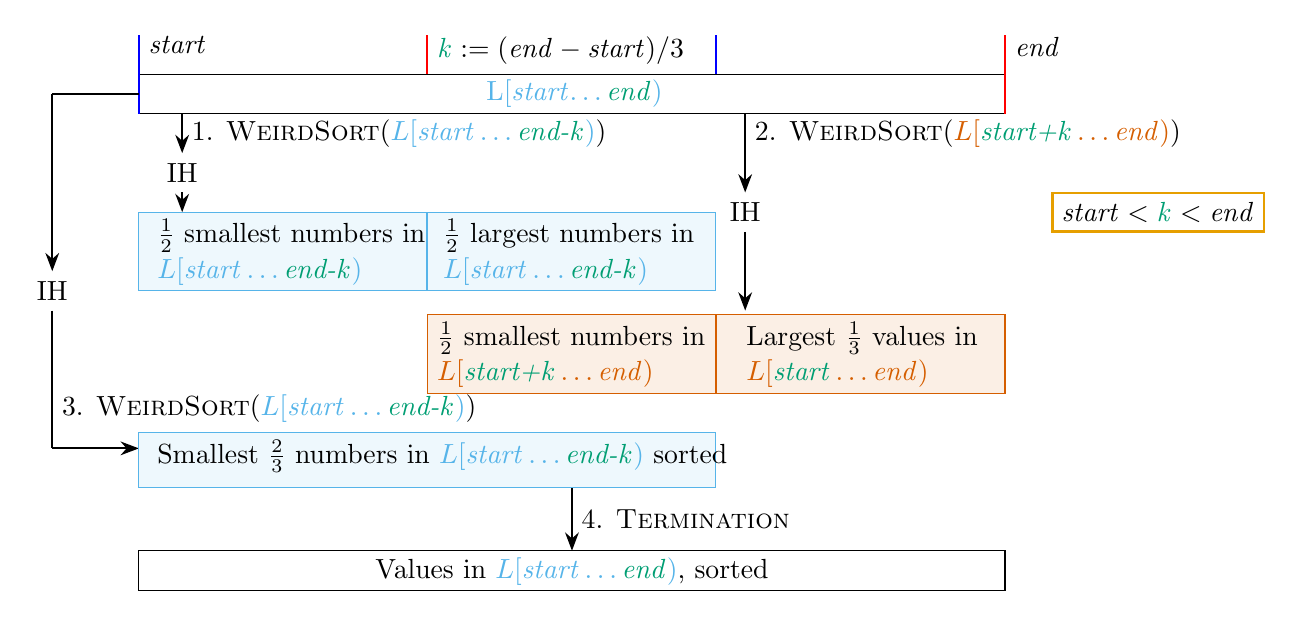
\begin{tikzpicture}[xscale=1.1]
    \draw (0, -0.25) rectangle (10, 0.25);
    \draw[thick, color=blue] (0, -0.25) -- (0, 0.75);
    \draw[thick, color=red] (10, -0.25) -- (10, 0.75);
    \node[below right] at (  0, 0.85) {\VAR{start}};
    \node[below right] at ( 10, 0.85) {\VAR{end}};

    \draw[thick, color=red] (3.33, 0.25) -- (3.33, 0.75);
    \draw[thick, color=blue] (6.66, 0.25) -- (6.66, 0.75);
    \node[below right] at (3.33, 0.85) {${\color{cbBluishGreen} \VAR{k}} \GETS (\VAR{end} - \VAR{start})/3$};

    \draw[thick,->] (0.5, -0.25) -- (0.5, -0.75);
    \node[right] at (0.5, -0.5) {1. $\AName{WeirdSort}({\color{cbSkyBlue} L[\VAR{start}\dots{\color{cbBluishGreen}\VAR{end-k}})})$};
    \draw[thick,->] (7, -0.25) -- (7, -1.25);
    \node[right] at (7, -0.5) {2. $\AName{WeirdSort}({\color{cbVermillion} L[{\color{cbBluishGreen}\VAR{start+k}}\dots\VAR{end})})$};

    \node[left,shape=rectangle,thick,draw,draw=cbOrange] at (13, -1.5) {$\VAR{start} < {\color{cbBluishGreen} \VAR{k}} < \VAR{end}$};

    \node at (0.5, -1) {IH};
    \node at (7, -1.5) {IH};

    \draw[thick,->] (0.5, -1.25) -- (0.5, -1.5);
    \draw[thick,->] (7, -1.75) -- (7, -2.75);

    \draw[cbSkyBlue,fill=cbSkyBlue!10] (0, -2.5) rectangle (6.66, -1.5);
    \node[right] at (0.1, -1.8) {$\frac{1}{2}$ smallest numbers in};
    \node[right] at (0.1, -2.25) {${\color{cbSkyBlue} L[\VAR{start}\dots{\color{cbBluishGreen}\VAR{end-k}})}$};

    \draw[thick, color=cbSkyBlue] (3.33, -1.5) -- (3.33, -2.5);

    \node[right] at (3.4, -1.8) {$\frac{1}{2}$ largest numbers in};
    \node[right] at (3.4, -2.25) {${\color{cbSkyBlue} L[\VAR{start}\dots{\color{cbBluishGreen}\VAR{end-k}})}$};
    
    
    % \node[right] at (0, -2.25) {where the largest $\frac{1}{3}$ values are at the end of the list};
    % \node[right] at (0, -2.75) {where the largest $\frac{1}{3}$ values are at the end of the list};

    \draw[cbVermillion,fill=cbVermillion!10] (3.33, -3.8) rectangle (10, -2.80);
    \node[right] at (3.33, -3.1) {$\frac{1}{2}$ smallest numbers in};
    \node[right] at (3.33, -3.55) {${\color{cbVermillion} L[{\color{cbBluishGreen}\VAR{start+k}}\dots\VAR{end})}$};

    \draw[thick, color=cbVermillion] (6.66, -2.8) -- (6.66, -3.8);

    \node[right] at (6.9, -3.1) {Largest $\frac{1}{3}$ values in};
    \node[right] at (6.9, -3.55) {${\color{cbVermillion} L[{\color{cbBluishGreen}\VAR{start}}\dots\VAR{end})}$};

    \node[right] at (3.9, 0) {{\color{cbSkyBlue} L[\VAR{start}\dots{\color{cbBluishGreen}\VAR{end}})}};

    \draw[thick] (0, 0) -- (-1, 0);
    \draw[thick,->] (-1, 0) -- (-1, -2.25);
    \node at (-1, -2.5) {IH};
    \draw[thick] (-1, -2.75) -- (-1, -4.5);
    \draw[thick,->] (-1, -4.5) -- (0, -4.5);
    \node[right] at (-1, -4) {3. $\AName{WeirdSort}({\color{cbSkyBlue} L[\VAR{start}\dots{\color{cbBluishGreen}\VAR{end-k}})})$};

    \draw[thick,->] (5, -5) -- (5, -5.8);
    \node[right] at (5, -5.4) {4. \AName{Termination}};
    

    \draw[cbSkyBlue,fill=cbSkyBlue!10] (0, -5) rectangle (6.66, -4.3);
    \node[right] at (0.1, -4.6) {Smallest $\frac{2}{3}$ numbers in ${\color{cbSkyBlue} L[\VAR{start}\dots{\color{cbBluishGreen}\VAR{end-k}})}$ sorted};

    % \draw[thick] (4.75, -1.75) -- (5.25, -1.75);
    % \draw[thick,->] (5, -1.75) -- (5, -3);
    % \node[right] at (5, -2.5) {\textcolor{cbReddischPurple}{Merge}};

    \draw (0, -5.8) rectangle (10, -6.3);
    % \node[left,shape=rectangle,thick,draw,draw=cbOrange] at (13.75, -2.5) {Assumption: \textcolor{cbReddischPurple}{WeirdSort} is correct};
    \node at (5, -6.07) {Values in ${\color{cbSkyBlue} L[\VAR{start}\dots{\color{cbBluishGreen}\VAR{end}})}$, sorted};
\end{tikzpicture}

Base case 1: $0<= end - start = 2$ values\\
In this case, it will hit the first if statement and sort the 2 values based on which is largest, then return. There is no recursion in this case.\\

Base case 2: $0<= end - start = 3$ values\\
This is the lowest amount of values where there will be recursion. This will result in $k = (3-0)/3 = 1$\\
Induction Hypothesis: WeirdSort sorts $0<= end - start < n$ values correct.\\
Induction Step: Prove WeirdSort sorts $end - start = n$ values\\

To start, assume $|L| = 3n, n \in \mathbb{N}, n > 0$ ($|L|$ is a multiple of 3). k will always give us $\frac{1}{3} |L|$, so each WeirdSort call will be $\frac{2}{3}$ of L. Since our base case 2 shows that $k>=1$ always, this means the lists drawn for the 3 WeirdSort calls will be at least 1 smaller than the input array. Given this, we can see that, assuming WeirdSort can sort $<n$ values via IH, WeirdSort call 1 will sort the largest $\frac{1}{3}$ values of L into the middle third of L (second half of L in WeirdSort call 1). WeirdSort call 2 will then take those largest numbers sorted in the first call and sort then with the remaining $\frac{1}{3}$ values. By the end of this call, the largest $\frac{1}{3}$ values in L will be sorted at the end of the list. WeirdSort call 3 will then sort the last (and smallest) $\frac{2}{3}$ values.\\

The following is looking at the case where the largest values are at the start of the list and the smallest at the end (assume reverse ordered list). You can see that there are enough of the largest values moved to the end of the first WeirdSort call, so that they can be sorted to the end of the list. This is because as seen by the final WeirdSort call, you only need to move the $\frac{1}{3}$ largest values to the last $\frac{2}{3}$ of the list, in order for them to be sorted to the end of the list. The final WeirdSort call will handle the rest.\\

Start of WeirdSort call 1\\
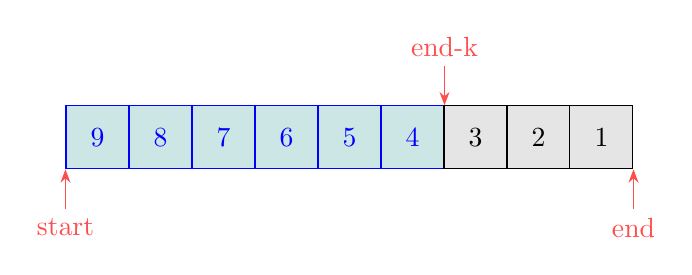
\begin{tikzpicture}
\matrix (A) [matrix of nodes, nodes={draw, minimum size=8mm},
    column sep=-\pgflinewidth,
    nodes={fill=gray!20},
    column 1/.style={blue, nodes={fill=teal!20}},
    column 2/.style={blue, nodes={fill=teal!20}},
    column 3/.style={blue, nodes={fill=teal!20}},
    column 4/.style={blue, nodes={fill=teal!20}},
    column 5/.style={blue, nodes={fill=teal!20}},
    column 6/.style={blue, nodes={fill=teal!20}},
    ]{
    9 & 8 & 7 & 6 & 5 & 4 & 3 & 2 & 1\\};

    \foreach \i [evaluate=\i as \ni using {int(\i)},
    evaluate=\i as \ntext using {"end-k"}] in {6}
    \draw [{Stealth}-, red!70] (A-1-\ni.north east)--++(90:5mm) node[above] {\ntext};
    
    \foreach \i [evaluate=\i as \ni using {int(\i)},
    evaluate=\i as \ntext using {"start"}] in {1}
    \draw [{Stealth}-, red!70] (A-1-\ni.south west)--++(-90:5mm) node[below] {\ntext};

    \foreach \i [evaluate=\i as \ni using {int(\i)},
    evaluate=\i as \ntext using {"end"}] in {9}
    \draw [{Stealth}-, red!70] (A-1-\ni.south east)--++(-90:5mm) node[below] {\ntext};

\end{tikzpicture}

End of WeirdSort call 1\\
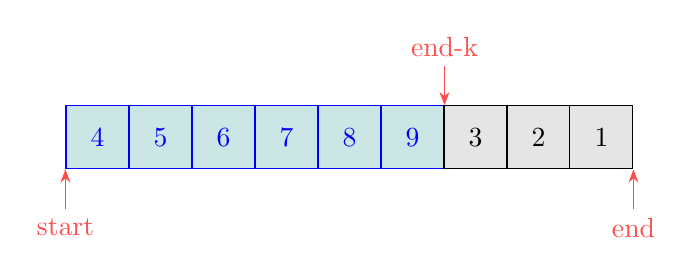
\begin{tikzpicture}
\matrix (A) [matrix of nodes, nodes={draw, minimum size=8mm},
    column sep=-\pgflinewidth,
    nodes={fill=gray!20},
    column 1/.style={blue, nodes={fill=teal!20}},
    column 2/.style={blue, nodes={fill=teal!20}},
    column 3/.style={blue, nodes={fill=teal!20}},
    column 4/.style={blue, nodes={fill=teal!20}},
    column 5/.style={blue, nodes={fill=teal!20}},
    column 6/.style={blue, nodes={fill=teal!20}},
    ]{
    4 & 5 & 6 & 7 & 8 & 9 & 3 & 2 & 1\\};

    \foreach \i [evaluate=\i as \ni using {int(\i)},
    evaluate=\i as \ntext using {"end-k"}] in {6}
    \draw [{Stealth}-, red!70] (A-1-\ni.north east)--++(90:5mm) node[above] {\ntext};
    
    \foreach \i [evaluate=\i as \ni using {int(\i)},
    evaluate=\i as \ntext using {"start"}] in {1}
    \draw [{Stealth}-, red!70] (A-1-\ni.south west)--++(-90:5mm) node[below] {\ntext};

    \foreach \i [evaluate=\i as \ni using {int(\i)},
    evaluate=\i as \ntext using {"end"}] in {9}
    \draw [{Stealth}-, red!70] (A-1-\ni.south east)--++(-90:5mm) node[below] {\ntext};

\end{tikzpicture}

Start of WeirdSort call 2\\
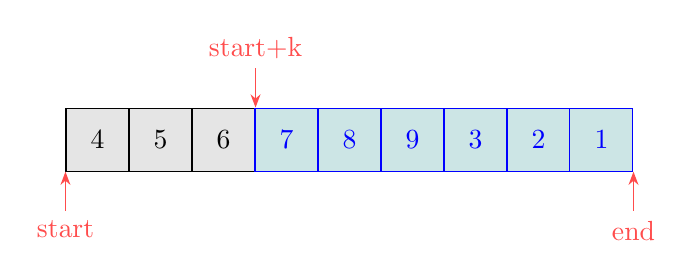
\begin{tikzpicture}
\matrix (A) [matrix of nodes, nodes={draw, minimum size=8mm},
    column sep=-\pgflinewidth,
    nodes={fill=gray!20},
    column 9/.style={blue, nodes={fill=teal!20}},
    column 8/.style={blue, nodes={fill=teal!20}},
    column 7/.style={blue, nodes={fill=teal!20}},
    column 4/.style={blue, nodes={fill=teal!20}},
    column 5/.style={blue, nodes={fill=teal!20}},
    column 6/.style={blue, nodes={fill=teal!20}},
    ]{
    4 & 5 & 6 & 7 & 8 & 9 & 3 & 2 & 1\\};

    \foreach \i [evaluate=\i as \ni using {int(\i)},
    evaluate=\i as \ntext using {"start+k"}] in {3}
    \draw [{Stealth}-, red!70] (A-1-\ni.north east)--++(90:5mm) node[above] {\ntext};
    
    \foreach \i [evaluate=\i as \ni using {int(\i)},
    evaluate=\i as \ntext using {"start"}] in {1}
    \draw [{Stealth}-, red!70] (A-1-\ni.south west)--++(-90:5mm) node[below] {\ntext};

    \foreach \i [evaluate=\i as \ni using {int(\i)},
    evaluate=\i as \ntext using {"end"}] in {9}
    \draw [{Stealth}-, red!70] (A-1-\ni.south east)--++(-90:5mm) node[below] {\ntext};

\end{tikzpicture}

End of WeirdSort call 2\\
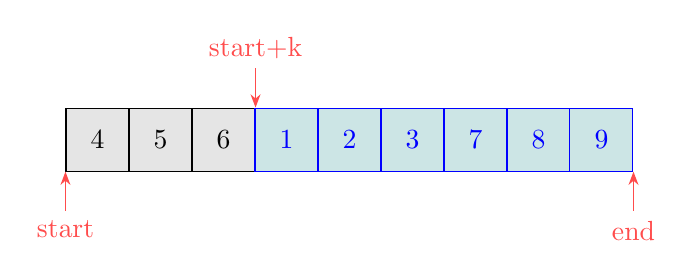
\begin{tikzpicture}
\matrix (A) [matrix of nodes, nodes={draw, minimum size=8mm},
    column sep=-\pgflinewidth,
    nodes={fill=gray!20},
    column 9/.style={blue, nodes={fill=teal!20}},
    column 8/.style={blue, nodes={fill=teal!20}},
    column 7/.style={blue, nodes={fill=teal!20}},
    column 4/.style={blue, nodes={fill=teal!20}},
    column 5/.style={blue, nodes={fill=teal!20}},
    column 6/.style={blue, nodes={fill=teal!20}},
    ]{
    4 & 5 & 6 & 1 & 2 & 3 & 7 & 8 & 9\\};

    \foreach \i [evaluate=\i as \ni using {int(\i)},
    evaluate=\i as \ntext using {"start+k"}] in {3}
    \draw [{Stealth}-, red!70] (A-1-\ni.north east)--++(90:5mm) node[above] {\ntext};
    
    \foreach \i [evaluate=\i as \ni using {int(\i)},
    evaluate=\i as \ntext using {"start"}] in {1}
    \draw [{Stealth}-, red!70] (A-1-\ni.south west)--++(-90:5mm) node[below] {\ntext};

    \foreach \i [evaluate=\i as \ni using {int(\i)},
    evaluate=\i as \ntext using {"end"}] in {9}
    \draw [{Stealth}-, red!70] (A-1-\ni.south east)--++(-90:5mm) node[below] {\ntext};

\end{tikzpicture}

Start of WeirdSort call 3\\
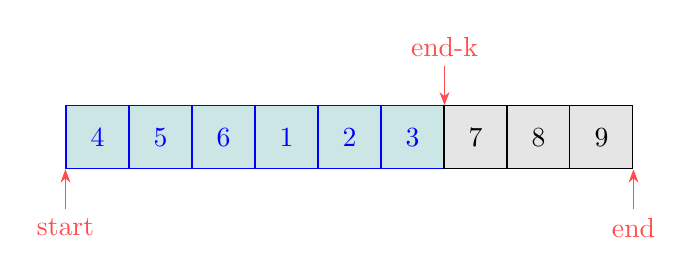
\begin{tikzpicture}
\matrix (A) [matrix of nodes, nodes={draw, minimum size=8mm},
    column sep=-\pgflinewidth,
    nodes={fill=gray!20},
    column 1/.style={blue, nodes={fill=teal!20}},
    column 2/.style={blue, nodes={fill=teal!20}},
    column 3/.style={blue, nodes={fill=teal!20}},
    column 4/.style={blue, nodes={fill=teal!20}},
    column 5/.style={blue, nodes={fill=teal!20}},
    column 6/.style={blue, nodes={fill=teal!20}},
    ]{
    4 & 5 & 6 & 1 & 2 & 3 & 7 & 8 & 9\\};

    \foreach \i [evaluate=\i as \ni using {int(\i)},
    evaluate=\i as \ntext using {"end-k"}] in {6}
    \draw [{Stealth}-, red!70] (A-1-\ni.north east)--++(90:5mm) node[above] {\ntext};
    
    \foreach \i [evaluate=\i as \ni using {int(\i)},
    evaluate=\i as \ntext using {"start"}] in {1}
    \draw [{Stealth}-, red!70] (A-1-\ni.south west)--++(-90:5mm) node[below] {\ntext};

    \foreach \i [evaluate=\i as \ni using {int(\i)},
    evaluate=\i as \ntext using {"end"}] in {9}
    \draw [{Stealth}-, red!70] (A-1-\ni.south east)--++(-90:5mm) node[below] {\ntext};

\end{tikzpicture}

End of WeirdSort call 3\\
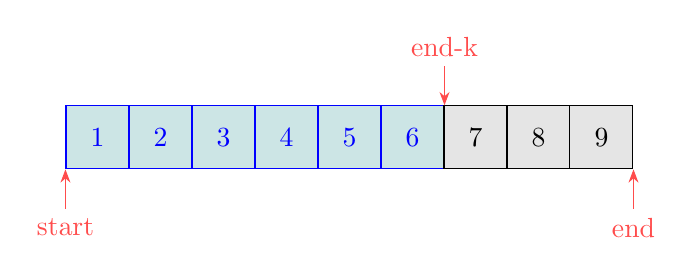
\begin{tikzpicture}
\matrix (A) [matrix of nodes, nodes={draw, minimum size=8mm},
    column sep=-\pgflinewidth,
    nodes={fill=gray!20},
    column 1/.style={blue, nodes={fill=teal!20}},
    column 2/.style={blue, nodes={fill=teal!20}},
    column 3/.style={blue, nodes={fill=teal!20}},
    column 4/.style={blue, nodes={fill=teal!20}},
    column 5/.style={blue, nodes={fill=teal!20}},
    column 6/.style={blue, nodes={fill=teal!20}},
    ]{
    1 & 2 & 3 & 4 & 5 & 6 & 7 & 8 & 9\\};

    \foreach \i [evaluate=\i as \ni using {int(\i)},
    evaluate=\i as \ntext using {"end-k"}] in {6}
    \draw [{Stealth}-, red!70] (A-1-\ni.north east)--++(90:5mm) node[above] {\ntext};
    
    \foreach \i [evaluate=\i as \ni using {int(\i)},
    evaluate=\i as \ntext using {"start"}] in {1}
    \draw [{Stealth}-, red!70] (A-1-\ni.south west)--++(-90:5mm) node[below] {\ntext};

    \foreach \i [evaluate=\i as \ni using {int(\i)},
    evaluate=\i as \ntext using {"end"}] in {9}
    \draw [{Stealth}-, red!70] (A-1-\ni.south east)--++(-90:5mm) node[below] {\ntext};

\end{tikzpicture}

Now given that $|L|$ is not a multiple of 3, there are two cases: $|L|=3n+1$ and $|L|=3n+2$. For both of these cases, there will be more values pushed to the end of the list in WeirdSort call 1, for WerirdSort call 2 to move to the end of the list. This is because k always rounds down, so the subsequent lists from WeirdSort calls will be bigger. More formally, for this to occur $|L[start+k,end-k)| >= L[end-k,end)$ An example can be seen below given\\

$|L|=3n+1$\\
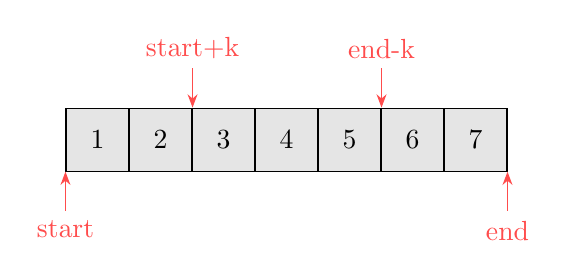
\begin{tikzpicture}
\matrix (A) [matrix of nodes, nodes={draw, minimum size=8mm},
    column sep=-\pgflinewidth,
    nodes={fill=gray!20},
    ]{
    1 & 2 & 3 & 4 & 5 & 6 & 7\\};

    \foreach \i [evaluate=\i as \ni using {int(\i)},
    evaluate=\i as \ntext using {"start+k"}] in {2}
    \draw [{Stealth}-, red!70] (A-1-\ni.north east)--++(90:5mm) node[above] {\ntext};
    
    \foreach \i [evaluate=\i as \ni using {int(\i)},
    evaluate=\i as \ntext using {"end-k"}] in {5}
    \draw [{Stealth}-, red!70] (A-1-\ni.north east)--++(90:5mm) node[above] {\ntext};
    
    \foreach \i [evaluate=\i as \ni using {int(\i)},
    evaluate=\i as \ntext using {"start"}] in {1}
    \draw [{Stealth}-, red!70] (A-1-\ni.south west)--++(-90:5mm) node[below] {\ntext};

    \foreach \i [evaluate=\i as \ni using {int(\i)},
    evaluate=\i as \ntext using {"end"}] in {7}
    \draw [{Stealth}-, red!70] (A-1-\ni.south east)--++(-90:5mm) node[below] {\ntext};

\end{tikzpicture}

$|L|=3n+2$\\
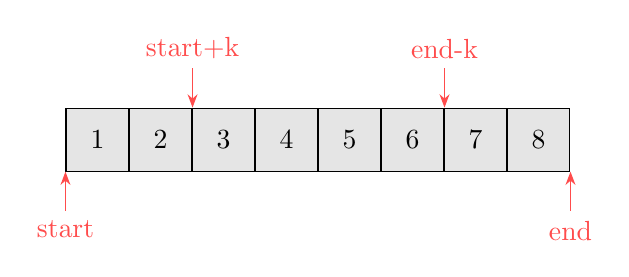
\begin{tikzpicture}
\matrix (A) [matrix of nodes, nodes={draw, minimum size=8mm},
    column sep=-\pgflinewidth,
    nodes={fill=gray!20},
    ]{
    1 & 2 & 3 & 4 & 5 & 6 & 7 & 8\\};

    \foreach \i [evaluate=\i as \ni using {int(\i)},
    evaluate=\i as \ntext using {"start+k"}] in {2}
    \draw [{Stealth}-, red!70] (A-1-\ni.north east)--++(90:5mm) node[above] {\ntext};
    
    \foreach \i [evaluate=\i as \ni using {int(\i)},
    evaluate=\i as \ntext using {"end-k"}] in {6}
    \draw [{Stealth}-, red!70] (A-1-\ni.north east)--++(90:5mm) node[above] {\ntext};
    
    \foreach \i [evaluate=\i as \ni using {int(\i)},
    evaluate=\i as \ntext using {"start"}] in {1}
    \draw [{Stealth}-, red!70] (A-1-\ni.south west)--++(-90:5mm) node[below] {\ntext};

    \foreach \i [evaluate=\i as \ni using {int(\i)},
    evaluate=\i as \ntext using {"end"}] in {8}
    \draw [{Stealth}-, red!70] (A-1-\ni.south east)--++(-90:5mm) node[below] {\ntext};

\end{tikzpicture}

\item Give a recurrence $T(n)$ for the runtime complexity of \AName{WeirdSort} and solve the recurrence $T(n)$ by proving that $T(n) \OOG{e(n)}$ for some expression $e$ that uses $n$.\\
\textbf{Answer:}\\

\begin{equation}
    T(N) = 
    \left\{
        \begin{array}{lr}
            0, & \text{if } N = 1\\ 
            1, & \text{if } N = 2\\
            T(\frac{2N}{3}) + T(\frac{2N}{3}) + T(\frac{2N}{3}) + 3, & \text{if } N > 2 
        \end{array}
    \right\}
\end{equation} \\

Using Master Theorem, we have $a=3$, $b=1.5$, $f(n)=3 \sim 1=N^{\log_{1.5}(1.5)}=\mathcal{O}(N^{\log_{1.5}(3-\epsilon)})$ where $\epsilon=1.5 > 0$, which is case 1 in Master Theorem. This means $T(N) \sim N^{\log_{1.5}(3)} \approx N^{2.71}$.

\end{questions}
\end{problem}

\begin{problem}
Consider the following \AName{Partition} algorithm used by \AName{QuickSort} (this version of \AName{Partition} is based on the algorithm from the slides with the for-loop replaced by a while-loop).
\begin{myalgo}{\AName{Partition}($L$, $\VAR{start}$, $\VAR{end}$)}
    \STATE $v, i, j \GETS L[\VAR{start}], \VAR{start}, \VAR{start + 1}$.
    \WHILE{$j \neq \VAR{end}$}\label{alg:while}
        \IF{$L[j] \leq v$}
            \STATE $i \GETS i + 1$.
            \STATE Exchange $L[i]$ and $L[j]$.
        \ENDIF
        \STATE $j \GETS j + 1$.
    \ENDWHILE
    \STATE Exchange $L[i]$ and $L[\VAR{start}]$
    \RETURN $i$.
\end{myalgo}

\begin{questions}
    \item Illustrate the operations performed by \AName{Partition} on the array $A = [21, 45, 7, 12, 28, 11, 17]$. Show the content of $A$ after each execution of the loop body.\\
\textbf{Answer:}\\
Start of function 

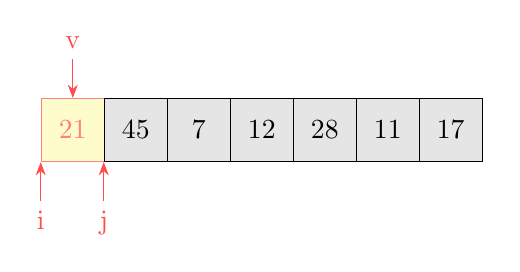
\begin{tikzpicture}
\matrix (A) [matrix of nodes, nodes={draw, minimum size=8mm},
    column sep=-\pgflinewidth,
    nodes={fill=gray!20},
    column 1/.style={red!50, nodes={fill=yellow!20}},]{
    21 & 45 & 7 & 12 & 28 & 11 & 17\\};

    \foreach \i [evaluate=\i as \ni using {int(\i)},
    evaluate=\i as \ntext using {"v"}] in {1}
    \draw [{Stealth}-, red!70] (A-1-\ni.north)--++(90:5mm) node[above] {\ntext};
    
    \foreach \i [evaluate=\i as \ni using {int(\i)},
    evaluate=\i as \ntext using {"i"}] in {1}
    \draw [{Stealth}-, red!70] (A-1-\ni.south west)--++(-90:5mm) node[below] {\ntext};

    \foreach \i [evaluate=\i as \ni using {int(\i)},
    evaluate=\i as \ntext using {"j"}] in {2}
    \draw [{Stealth}-, red!70] (A-1-\ni.south west)--++(-90:5mm) node[below] {\ntext};

\end{tikzpicture}
\\

Start of loop\\\\
Did not enter if statement\\
End Loop 1\\
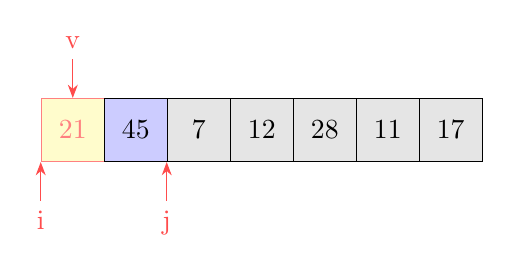
\begin{tikzpicture}
\matrix (A) [matrix of nodes, nodes={draw, minimum size=8mm},
    column sep=-\pgflinewidth,
    nodes={fill=gray!20},
    column 1/.style={red!50, nodes={fill=yellow!20}},
    column 2/.style={black, nodes={fill=blue!20}},
    ]{
    21 & 45 & 7 & 12 & 28 & 11 & 17\\};

    \foreach \i [evaluate=\i as \ni using {int(\i)},
    evaluate=\i as \ntext using {"v"}] in {1}
    \draw [{Stealth}-, red!70] (A-1-\ni.north)--++(90:5mm) node[above] {\ntext};
    
    \foreach \i [evaluate=\i as \ni using {int(\i)},
    evaluate=\i as \ntext using {"i"}] in {1}
    \draw [{Stealth}-, red!70] (A-1-\ni.south west)--++(-90:5mm) node[below] {\ntext};

    \foreach \i [evaluate=\i as \ni using {int(\i)},
    evaluate=\i as \ntext using {"j"}] in {3}
    \draw [{Stealth}-, red!70] (A-1-\ni.south west)--++(-90:5mm) node[below] {\ntext};

\end{tikzpicture}

Entered if statement\\
End Loop 2\\
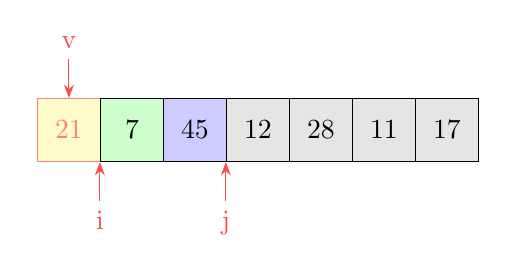
\begin{tikzpicture}
\matrix (A) [matrix of nodes, nodes={draw, minimum size=8mm},
    column sep=-\pgflinewidth,
    nodes={fill=gray!20},
    column 1/.style={red!50, nodes={fill=yellow!20}},
    column 2/.style={black, nodes={fill=green!20}},
    column 3/.style={black, nodes={fill=blue!20}},]{
    21 & 7 & 45 & 12 & 28 & 11 & 17\\};
    
    \foreach \i [evaluate=\i as \ni using {int(\i)},
    evaluate=\i as \ntext using {"v"}] in {1}
    \draw [{Stealth}-, red!70] (A-1-\ni.north)--++(90:5mm) node[above] {\ntext};
    
    \foreach \i [evaluate=\i as \ni using {int(\i)},
    evaluate=\i as \ntext using {"i"}] in {2}
    \draw [{Stealth}-, red!70] (A-1-\ni.south west)--++(-90:5mm) node[below] {\ntext};

    \foreach \i [evaluate=\i as \ni using {int(\i)},
    evaluate=\i as \ntext using {"j"}] in {4}
    \draw [{Stealth}-, red!70] (A-1-\ni.south west)--++(-90:5mm) node[below] {\ntext};

\end{tikzpicture}

Entered if statement\\
End Loop 3\\
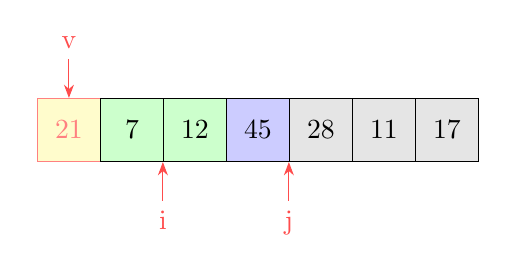
\begin{tikzpicture}
\matrix (A) [matrix of nodes, nodes={draw, minimum size=8mm},
    column sep=-\pgflinewidth,
    nodes={fill=gray!20},
    column 1/.style={red!50, nodes={fill=yellow!20}},
    column 2/.style={black, nodes={fill=green!20}},
    column 3/.style={black, nodes={fill=green!20}},
    column 4/.style={black, nodes={fill=blue!20}},]{
    21 & 7 & 12 & 45 & 28 & 11 & 17\\};

    \foreach \i [evaluate=\i as \ni using {int(\i)},
    evaluate=\i as \ntext using {"v"}] in {1}
    \draw [{Stealth}-, red!70] (A-1-\ni.north)--++(90:5mm) node[above] {\ntext};
    
    \foreach \i [evaluate=\i as \ni using {int(\i)},
    evaluate=\i as \ntext using {"i"}] in {3}
    \draw [{Stealth}-, red!70] (A-1-\ni.south west)--++(-90:5mm) node[below] {\ntext};

    \foreach \i [evaluate=\i as \ni using {int(\i)},
    evaluate=\i as \ntext using {"j"}] in {5}
    \draw [{Stealth}-, red!70] (A-1-\ni.south west)--++(-90:5mm) node[below] {\ntext};

\end{tikzpicture}

Did not enter if statement\\
End Loop 4\\
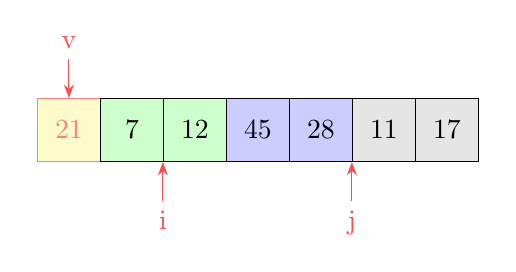
\begin{tikzpicture}
\matrix (A) [matrix of nodes, nodes={draw, minimum size=8mm},
    column sep=-\pgflinewidth,
    nodes={fill=gray!20},
    column 1/.style={red!50, nodes={fill=yellow!20}},
    column 2/.style={black, nodes={fill=green!20}},
    column 3/.style={black, nodes={fill=green!20}},
    column 4/.style={black, nodes={fill=blue!20}},
    column 5/.style={black, nodes={fill=blue!20}},]{
    21 & 7 & 12 & 45 & 28 & 11 & 17\\};

    \foreach \i [evaluate=\i as \ni using {int(\i)},
    evaluate=\i as \ntext using {"v"}] in {1}
    \draw [{Stealth}-, red!70] (A-1-\ni.north)--++(90:5mm) node[above] {\ntext};
    
    \foreach \i [evaluate=\i as \ni using {int(\i)},
    evaluate=\i as \ntext using {"i"}] in {3}
    \draw [{Stealth}-, red!70] (A-1-\ni.south west)--++(-90:5mm) node[below] {\ntext};

    \foreach \i [evaluate=\i as \ni using {int(\i)},
    evaluate=\i as \ntext using {"j"}] in {6}
    \draw [{Stealth}-, red!70] (A-1-\ni.south west)--++(-90:5mm) node[below] {\ntext};

\end{tikzpicture}

Entered if statement\\
End Loop 5\\
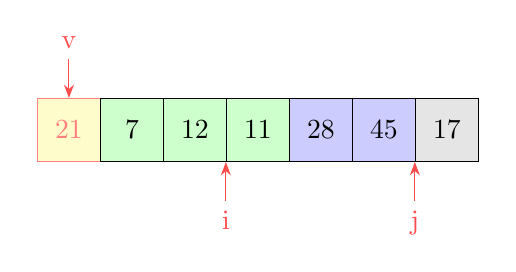
\begin{tikzpicture}
\matrix (A) [matrix of nodes, nodes={draw, minimum size=8mm},
    column sep=-\pgflinewidth,
    nodes={fill=gray!20},
    column 1/.style={red!50, nodes={fill=yellow!20}},
    column 2/.style={black, nodes={fill=green!20}},
    column 3/.style={black, nodes={fill=green!20}},
    column 4/.style={black, nodes={fill=green!20}},
    column 5/.style={black, nodes={fill=blue!20}},
    column 6/.style={black, nodes={fill=blue!20}},]{
    21 & 7 & 12 & 11 & 28 & 45 & 17\\};
    
    \foreach \i [evaluate=\i as \ni using {int(\i)},
    evaluate=\i as \ntext using {"v"}] in {1}
    \draw [{Stealth}-, red!70] (A-1-\ni.north)--++(90:5mm) node[above] {\ntext};

    \foreach \i [evaluate=\i as \ni using {int(\i)},
    evaluate=\i as \ntext using {"i"}] in {4}
    \draw [{Stealth}-, red!70] (A-1-\ni.south west)--++(-90:5mm) node[below] {\ntext};

    \foreach \i [evaluate=\i as \ni using {int(\i)},
    evaluate=\i as \ntext using {"j"}] in {7}
    \draw [{Stealth}-, red!70] (A-1-\ni.south west)--++(-90:5mm) node[below] {\ntext};

\end{tikzpicture}

Entered if statement\\
End Loop 6\\
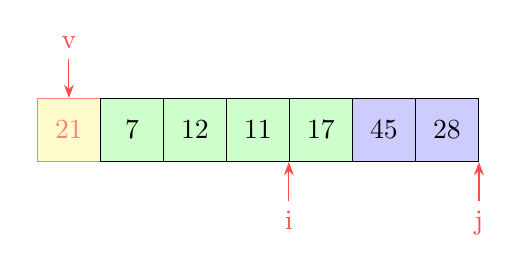
\begin{tikzpicture}
\matrix (A) [matrix of nodes, nodes={draw, minimum size=8mm},
    column sep=-\pgflinewidth,
    nodes={fill=gray!20},
    column 1/.style={red!50, nodes={fill=yellow!20}},
    column 2/.style={black, nodes={fill=green!20}},
    column 3/.style={black, nodes={fill=green!20}},
    column 4/.style={black, nodes={fill=green!20}},
    column 5/.style={black, nodes={fill=green!20}},
    column 6/.style={black, nodes={fill=blue!20}},
    column 7/.style={black, nodes={fill=blue!20}},]{
    21 & 7 & 12 & 11 & 17 & 45 & 28\\};

    \foreach \i [evaluate=\i as \ni using {int(\i)},
    evaluate=\i as \ntext using {"v"}] in {1}
    \draw [{Stealth}-, red!70] (A-1-\ni.north)--++(90:5mm) node[above] {\ntext};
    
    \foreach \i [evaluate=\i as \ni using {int(\i)},
    evaluate=\i as \ntext using {"i"}] in {5}
    \draw [{Stealth}-, red!70] (A-1-\ni.south west)--++(-90:5mm) node[below] {\ntext};

    \foreach \i [evaluate=\i as \ni using {int(\i)},
    evaluate=\i as \ntext using {"j"}] in {7}
    \draw [{Stealth}-, red!70] (A-1-\ni.south east)--++(-90:5mm) node[below] {\ntext};

\end{tikzpicture}
\\
End of loop\\
Exchange L[i] and L[start]\\
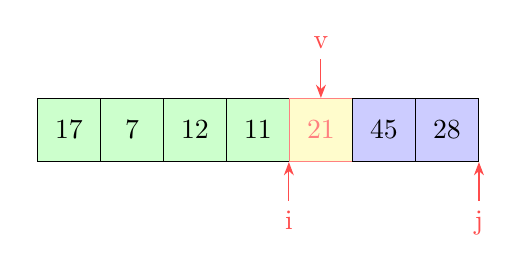
\begin{tikzpicture}
\matrix (A) [matrix of nodes, nodes={draw, minimum size=8mm},
    column sep=-\pgflinewidth,
    nodes={fill=gray!20},
    column 5/.style={red!50, nodes={fill=yellow!20}},
    column 2/.style={black, nodes={fill=green!20}},
    column 3/.style={black, nodes={fill=green!20}},
    column 4/.style={black, nodes={fill=green!20}},
    column 1/.style={black, nodes={fill=green!20}},
    column 6/.style={black, nodes={fill=blue!20}},
    column 7/.style={black, nodes={fill=blue!20}},]{
    17 & 7 & 12 & 11 & 21 & 45 & 28\\};

    \foreach \i [evaluate=\i as \ni using {int(\i)},
    evaluate=\i as \ntext using {"v"}] in {5}
    \draw [{Stealth}-, red!70] (A-1-\ni.north)--++(90:5mm) node[above] {\ntext};
    
    \foreach \i [evaluate=\i as \ni using {int(\i)},
    evaluate=\i as \ntext using {"i"}] in {5}
    \draw [{Stealth}-, red!70] (A-1-\ni.south west)--++(-90:5mm) node[below] {\ntext};

    \foreach \i [evaluate=\i as \ni using {int(\i)},
    evaluate=\i as \ntext using {"j"}] in {7}
    \draw [{Stealth}-, red!70] (A-1-\ni.south east)--++(-90:5mm) node[below] {\ntext};

\end{tikzpicture}


    \item Provide pre-conditions and post-conditions for \AName{Partition} and provide an invariant and bound function for the while-loop at Line~\ref*{alg:while}. Prove the correctness of \AName{Partition}.\\
Pre-condition:
\begin{enumerate}
    \item[-] $|L| > 0$, else L[start] would error
\end{enumerate}
Post-condition:
\begin{enumerate}
    \item[-] All elements to the left of v are smaller than or equal to v, all elements to the right of v are larger than v, v is in the middle of the smaller and larger elements.
    \item[-] The input array is the same length as the output array and contains the same values (not necessarily in the same order)
\end{enumerate}
Loop Invariant:
\begin{enumerate}
    \item[-] All entries in A[$start+1$...$i$] are $<=$ pivot.
    \item[-] All entries in A[$i + 1$...$j$) are $>$ pivot.
    \item[-] A[start] = pivot.
\end{enumerate}
Bound function:
\begin{enumerate}
    \item[-] $end-j$, this is because when $end = j$, this means $end-j=0$ and the loop will terminate
\end{enumerate}

\begin{myalgo}{\AName{Partition}($L$, $\VAR{start}$, $\VAR{end}$)}
    \STATE $v, i, j \GETS L[\VAR{start}], \VAR{start}, \VAR{start + 1}$.\\
    Base case: v=L[start] (pivot) and i=0 and j=1 implies invariant (L1 and L2 are both empty because their range is out of bounds) \\
    Given the invariant is: \\
    All entries in L1 = L[$start+1$...$i$] are $<=$ pivot.\\
    All entries in L2 = L[$i + 1$...$j$) are $>$ pivot.\\
    Induction hypothesis: The invariant holds at every step in the loop.\\
    Induction step: Prove that the invariant holds at every step in the loop.\\
    \WHILE{$j \neq \VAR{end}$}\label{alg:while}
    \STATE Known: $j \neq end$
        \IF{$L[j] \leq v$}
            \STATE $i \GETS i + 1$.
            \STATE Known: $L[j] \leq pivot$, L[$i_{new}$] is $\geq$ pivot because $i_{old}$ is always 1 cell behind the first element in L1
            \STATE Exchange $L[i]$ and $L[j]$.
            \STATE Known: j isn't at end of list yet. L[$start+1$...$i$] are all smaller than or equal to pivot and L[$i + 1$...$j-1$) are all larger than pivot 
    
        \ENDIF
        \STATE $j \GETS j + 1$.
        \STATE $j_{new} = j_{old} + 1$ meaning L[$i + 1$...$j_{new}$) are all larger than pivot, which is our invariant.
    \ENDWHILE
    \STATE Known: We know that L[$start+1$...$i$] are all smaller or equal to pivot and L[$i + 1$...$j$) are all larger than pivot. We know that the $i^{th}$ value is the last value included in L1 and everything past the $i^{th}$ value is part of L2, so we can swap it with the start value (pivot), making the new list have all smaller or equal values to the left of the pivot and all larger to the right.
    \STATE Exchange $L[i]$ and $L[\VAR{start}]$
    \\Known: L is a list where L[start...i) values are smaller than or equal to the pivot, L[i] is the pivot value, L[i+1...end) are all values larger than pivot.
    \RETURN $i$.
\end{myalgo}

    \item Argue how \AName{Partition} can be adjusted to run on singly linked lists $L$, while keeping a running time of $\OOG{\abs{L}}$.\\

\textbf{Answer:}\\
There are two methods to do this, both with the same thought process. (i) Exchange just the data between nodes. (ii) Exchange the actual nodes.\\

(i) Instead of holding the index i and j, we need to hold the nodes at position i and j. v can still be the data in the head node. To start, i would hold node 1, and j would hold node 2. As you are iterating through the loop, the comparison will need to be between v and j.data. If needing to exchange the nodes, you can just exchange the data, which is a constant time operation (3 ops to be specific). The while condition would now be j.next $\neq$ null as that specifies when you are at the last node. Whenever, there is an i++ or j++, that can be changed to node.next, which is also constant time. Finally, the final exchange at the end of the loop, is also a constant time function, as aforementioned. We would still need to hold a variable p that holds the index of the pivot (previous i), that will increment by 1 every time you call node.next on the ith node. This is because the index of the pivot needs to be returned at the end. This again is constant time as it is just incrementing an integer at max once per loop. Due to everything being constant time, while we loop through the whole list (N elements), this gives us $\sim L$ time complexity.\\

(ii) Instead of holding the index i and j, we need to hold the nodes right before position i and j. Holding the node before is since for a singly linked list, you can't go back, so you need to always have a reference (node.next) to the node you want to compare and swap. We also need a function to swap two nodes in the linked list. This function is constant time as it is just a few assignments. As exchanges only happen between nodes i and j, it is sufficient to keep track of only these nodes, while updating them by calling node.next whenever we need to do i++ or j++. This way, we can traverse the list once while using constant time functions in each iteration, giving us a complexity of $\sim L$.\\

The while loop condition would now need to be when j.next.next = null as that is when we've reached the second last node in the list. This is when we want to terminate since we are always holding the node one before the one we want to compare (index j-1). Furthermore as mentioned in (i), we would need to hold a new variable p that holds the index of the ith node so we can return it at the end. As argued above, it is constant time, so it won't affect the time complexity.\\

Note: You don't need to hold the node at v as we only need the value for comparisons during the loop, and you can quickly access the head of a linked list when it comes to getting the value of the head at the start and exchanging it at the end of the function.
\end{questions}
\end{problem}

\begin{problem}
Consider pairs $(x_i, y_i)$ such that $x_i$ is the time at which person $i = 0, 1, 2 , \dots$ enters the museum and $y_i$ is the time at which person $i$ leaves the museum.  You may assume that consecutive people enter the museum in order of increasing time ($x_0 \leq x_1 \leq \dots$).
\begin{questions}
\item Provide an algorithm \AName{MaxVisitors} that takes as input $L = [(x_0, y_0), \dots, (x_{N-1}, y_{N-1})]$ and computes in $\OOG{N \log N}$ the maximum number of visitors in the museum at any time.\\
\textbf{Answer:}\\

\begin{myalgo}{\AName{MaxVisitors}($L$)}
    \STATE $sortedL \GETS MergeSort(L)$ --> Assumption: MergeSort is correct, and returns a list where $x_i$ and $y_i$ are separate values, thus don't need to be consecutive. Both $x_i$ and $y_i$ have a flag that can tell if it is an entering or leaving time (ex. using a tuple (time, flag))\\
    \STATE $bst \GETS BuildBinarySearchTree(L)$ --> Nodes in binary tree have node.value = time and node.flag = enter or leave
    \STATE function $InOrderTraverse$(Node n, int currentVisitors, int maxVisitors) \{
        \IF{n.left $\neq$ @null}
            \STATE $InOrderTraverse$(n.left, currentVisitors, maxVisitors)
        \ENDIF
        \IF{$(n.flag == enter)$}
            \STATE $currentVisitors++$
        \ELSIF{$(n.flag == leave)$} 
            \STATE $currentVisitors--$
        \ENDIF
        \IF{$(maxVisitors < currentVisitors)$}
            \STATE $maxVisitors \GETS currentVisitors$
        \ENDIF
        \IF{n.right $\neq$ @null}
            \STATE $InOrderTraverse$(n.right, currentVisitors, maxVisitors)
        \ENDIF
        \RETURN maxVisitors
    \STATE $\}$ --> Assume when the function updates currentVisitors or maxVisitors, it updates it in main memory, so all recursions are updating the same location in memory. (ex. of this is giving the addresses of currentVisitors and maxVisitors) 
    \STATE $maxVisitors \GETS InOrderTraverse(bst, 0, 0)$ --> InOrder traverses the binary tree and adds 1 to currentVisitors when someone enters or removes 1 when someone leaves. It keeps track of the maximum value throughout the whole traversal and returns that number. 
    \RETURN $maxVisitors$.
\end{myalgo}

\item Argue why your algorithm \AName{MaxVisitors} is correct and has a runtime complexity of $\OOG{N \log N}$.

\item Assume that the museum has a maximum capacity of $M$. Provide a datastructure with an operation \AName{PersonEnters}($x_i$, $y_i$) that computes in at-most $\OOG{\log M}$ the number of visitors in the museum when person $i$ enters the museum (for any number of persons).

\item Argue why your algorithm \AName{PersonEnters} is correct and has a runtime complexity of $\OOG{\log M}$.

LOOK INTO MAX HEAP

\end{questions}

\end{problem}


\SUBMITMSG{}
\DEFAULTGRADING{}

\end{document}